\subsection{Overview}
% High-level components and their interaction% High-level components and their interaction
The application is divided in three logical layers:
\subsubsection{Presentation layer}
The presentation layer occupies the top level and displays information related to the services available on the CLup application in the form of an intuitive graphical user interface.
It constitutes the front-end layer of the application and the interface with which end-users will interact through a web-based application.
For example: if a user wants to schedule a visit to the store they can do so by selecting the schedule button on the main page, which is a part of the presentation layer.
The logic behind opening a new graphical interface for the user to select the exact store, date, day, and other preferences is a part of the application layer.
\subsubsection{Application layer}
The application layer coordinates the application, processes user requests, makes logical and business decisions, and performs calculations.
This layer is in charge of the workflows by which the data and requests travel, starting from the input received from the presentation layer
to the data layer alongside the business logic on the data collected.
In this project, the application layer resides on the server-side, meaning that all the computing is done outside the user scope.
For example: if a user wants to enter the store they can do so by showing the clerk a QR code that contains information about their visit time.
The clerk then proceeds to scan the user QR code and after successfully scanning it, the application layer residing on the server-side processes
the clerk request and responds to the clerk, furthermore to the presentation layer with a message whether or not a user is permitted to enter the store.
\subsubsection{Data layer}
The data layer is a centralized location that receives all data calls and provides access to the persistent storage of an application.
The data layer is closely connected to the business layer, so the logic knows which database to talk to and the data retrieving process is more optimized.
%Is the data layer divided somehow?
For example: when a user requests to schedule a visit time for a certain store, all available time slots are calculated from the data stored in the database.
That data is then processed using the application layer to the presentation layer and shown to the user.

Described architecture is a thin client architecture, in which the server does most of the work, which includes performing calculations and storing data.
\begin{figure}[H]
    \centering
    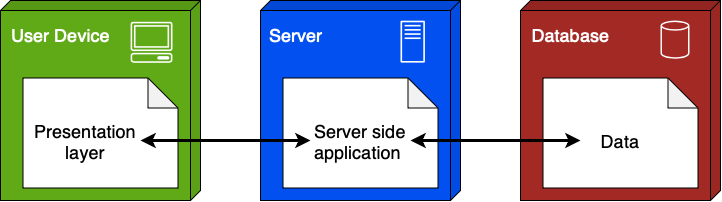
\includegraphics[height=0.7\textwidth]{Images/Overview.png}
    \caption{High level component architecture}
\end{figure}
%Need some more explaining on this part, I dont know what more to write about here :(


\subsection{Component view}
In the following section, components used to implement different functionalities of the system is described, aided with component diagrams demonstrating their separation and interactions within each other and with other external interfaces.
\begin{figure}[H]
    \centering
    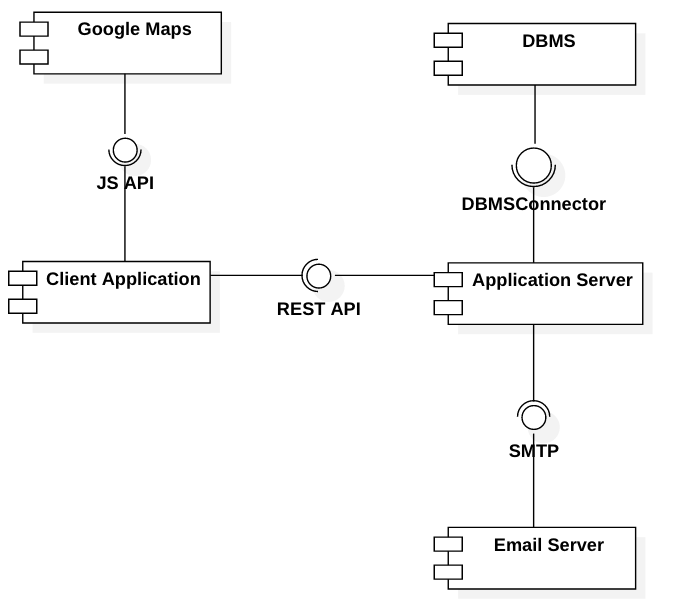
\includegraphics[height=0.4\textwidth]{Images/ComponentDiagrams/Overall.png}
    \caption{Component Diagram for the overall system}
    \label{fig:CDOverall}
\end{figure}
\nameref{fig:CDOverall} provides an overall view to the components present in the system and the connections between these components to correctly realize the decisions provided in this document.
The external integrations of the system, with the general communication interfaces they communicate with other components are provided, however the details for the Application Server will be presented following, only, considering that the main application logic is executed through the components residing in it.
The client is a thin-client built to interact with and display information directly sent through the endpoints.
Therefore, it is provided as one component that is unnecessary to split into sub-components.
\begin{figure}[H]
    \centering
    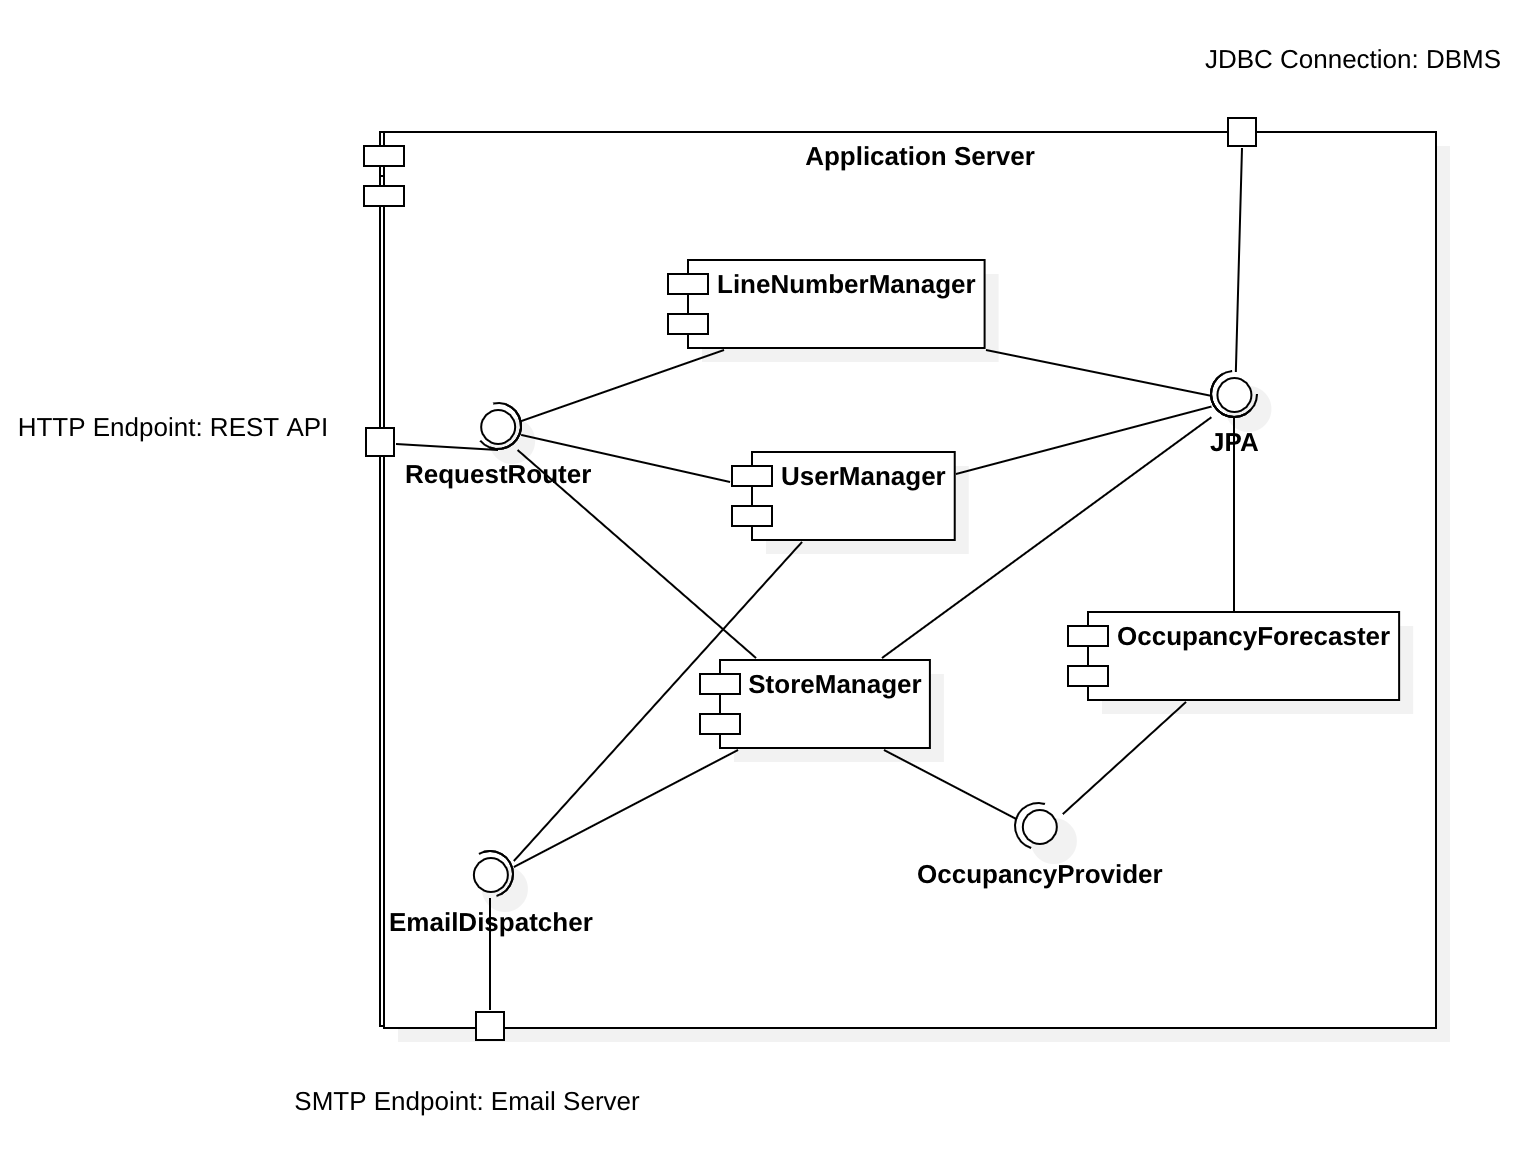
\includegraphics[height=0.4\textwidth]{Images/ComponentDiagrams/ApplicationServer.png}
    \caption{Component Diagram for the Application Server}
    \label{fig:CDApplicationServer}
\end{figure}
\nameref{fig:CDApplicationServer} provides an overall view for the components inside the Application Server.
The components separate the functionality into three domains, namely Line Numbers, Users and Stores.
All other entities that exist in the system are included into one of these domains based on their relevance.
All the user facing functionalities of the system are exposed through the REST endpoint, which uses a router interface to route each request to the domain component it belongs to.
All domain components use JPA to persist their domain data structures, and components that require to send e-mails use the SMTP endpoint to do so.
The OccupancyForecaster is a component that features only one function: periodically reading the database for entry and exit records of customers and updating the store accordingly.
Therefore, it is not split further into components.
\begin{figure}[H]
    \centering
    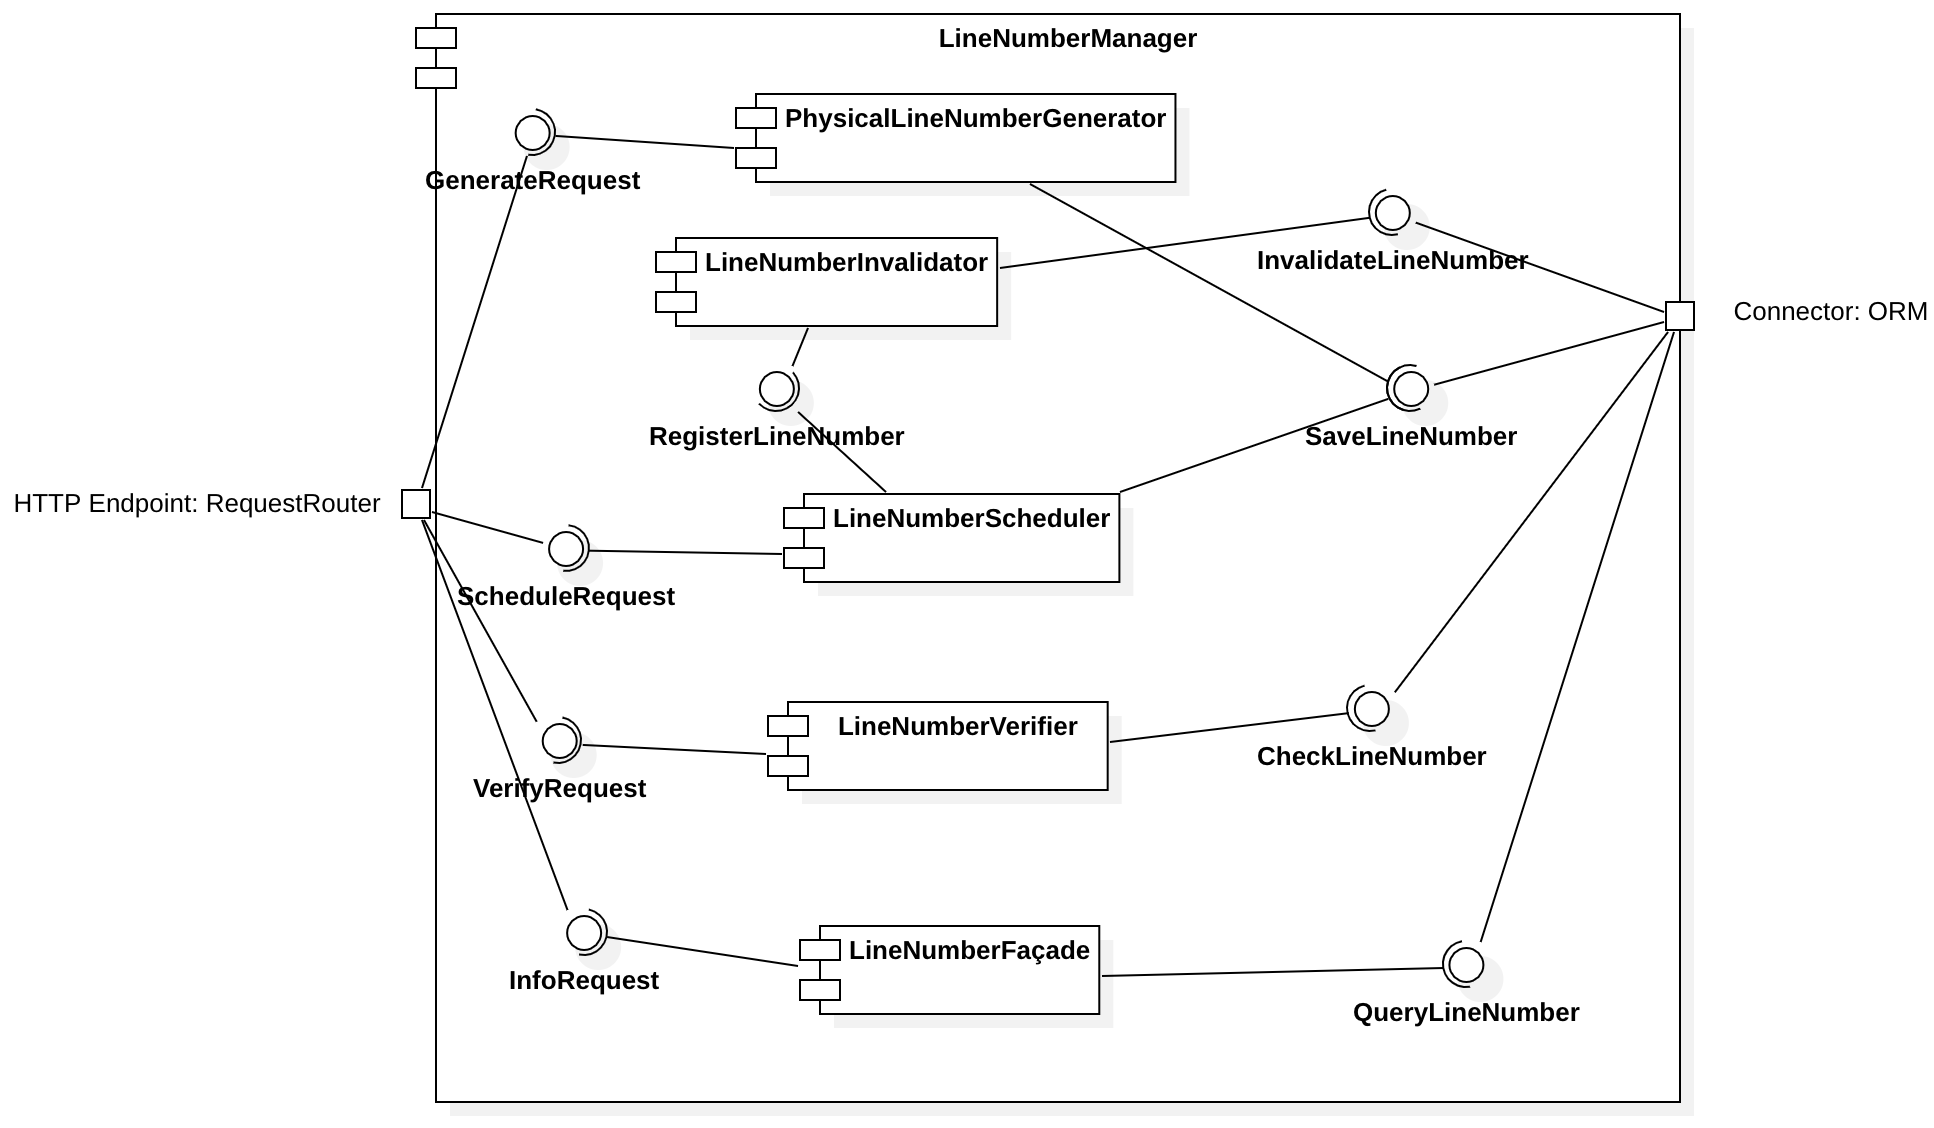
\includegraphics[height=0.4\textwidth]{Images/ComponentDiagrams/LineNumberManager.png}
    \caption{Component Diagram for the LineNumberManager}
    \label{fig:CDLineNumberManager}
\end{figure}
\nameref{fig:CDLineNumberManager} provides a detailed view over the domain component for line numbers.
It allows the management of any sort of query related to line numbers by clerks and customers.
This component is further divided into following sub-components to increase the granularity of actions performed on line numbers:
\begin{itemize}
    \item \textbf{PhysicalLineNumberGenerator}: This component exists to provide an interface for clerks to generate line numbers, it's interface handles the incoming request by generating and persisting a new ticket for the to-be-printed line number.
    \item \textbf{LineNumberScheduler}: This component exists to allow the users of the system to book a line number from their home.
    It realizes its functionality through connecting to the same interface of the persistence provider, however it is capable of handling more complex requests, including custom product or category selection and time slot allocation.
    Furthermore, it registers the ticket to the LineNumberInvalidator to be invalidated after the set timeout minutes have passed from the time slot.
    \item \textbf{LineNumberInvalidator}: This component acts as a helper component to LineNumberScheduler.
    It schedules the invalidation of the scheduled tickets, so that the invalidation can occur asynchronously.
    This component is created to separate this responsibility from an active user facing component, all which have the main responsibility to provide a synchronous response to all the users' needs.
    \item \textbf{LineNumberVerifier}: This component is used to handle the transactions regarding customer QR code verification conducted by the Clerk.
    It is used to register the entrance and exit of customers with their QR codes.
    \item \textbf{LineNumberFa\c{c}ade}: This component is used by the customers that want to query detailed information regarding the line numbers that they have.
    The requests handled by this endpoint is directly mapped to the client application's needs.

\end{itemize}
\begin{figure}[H]
    \centering
    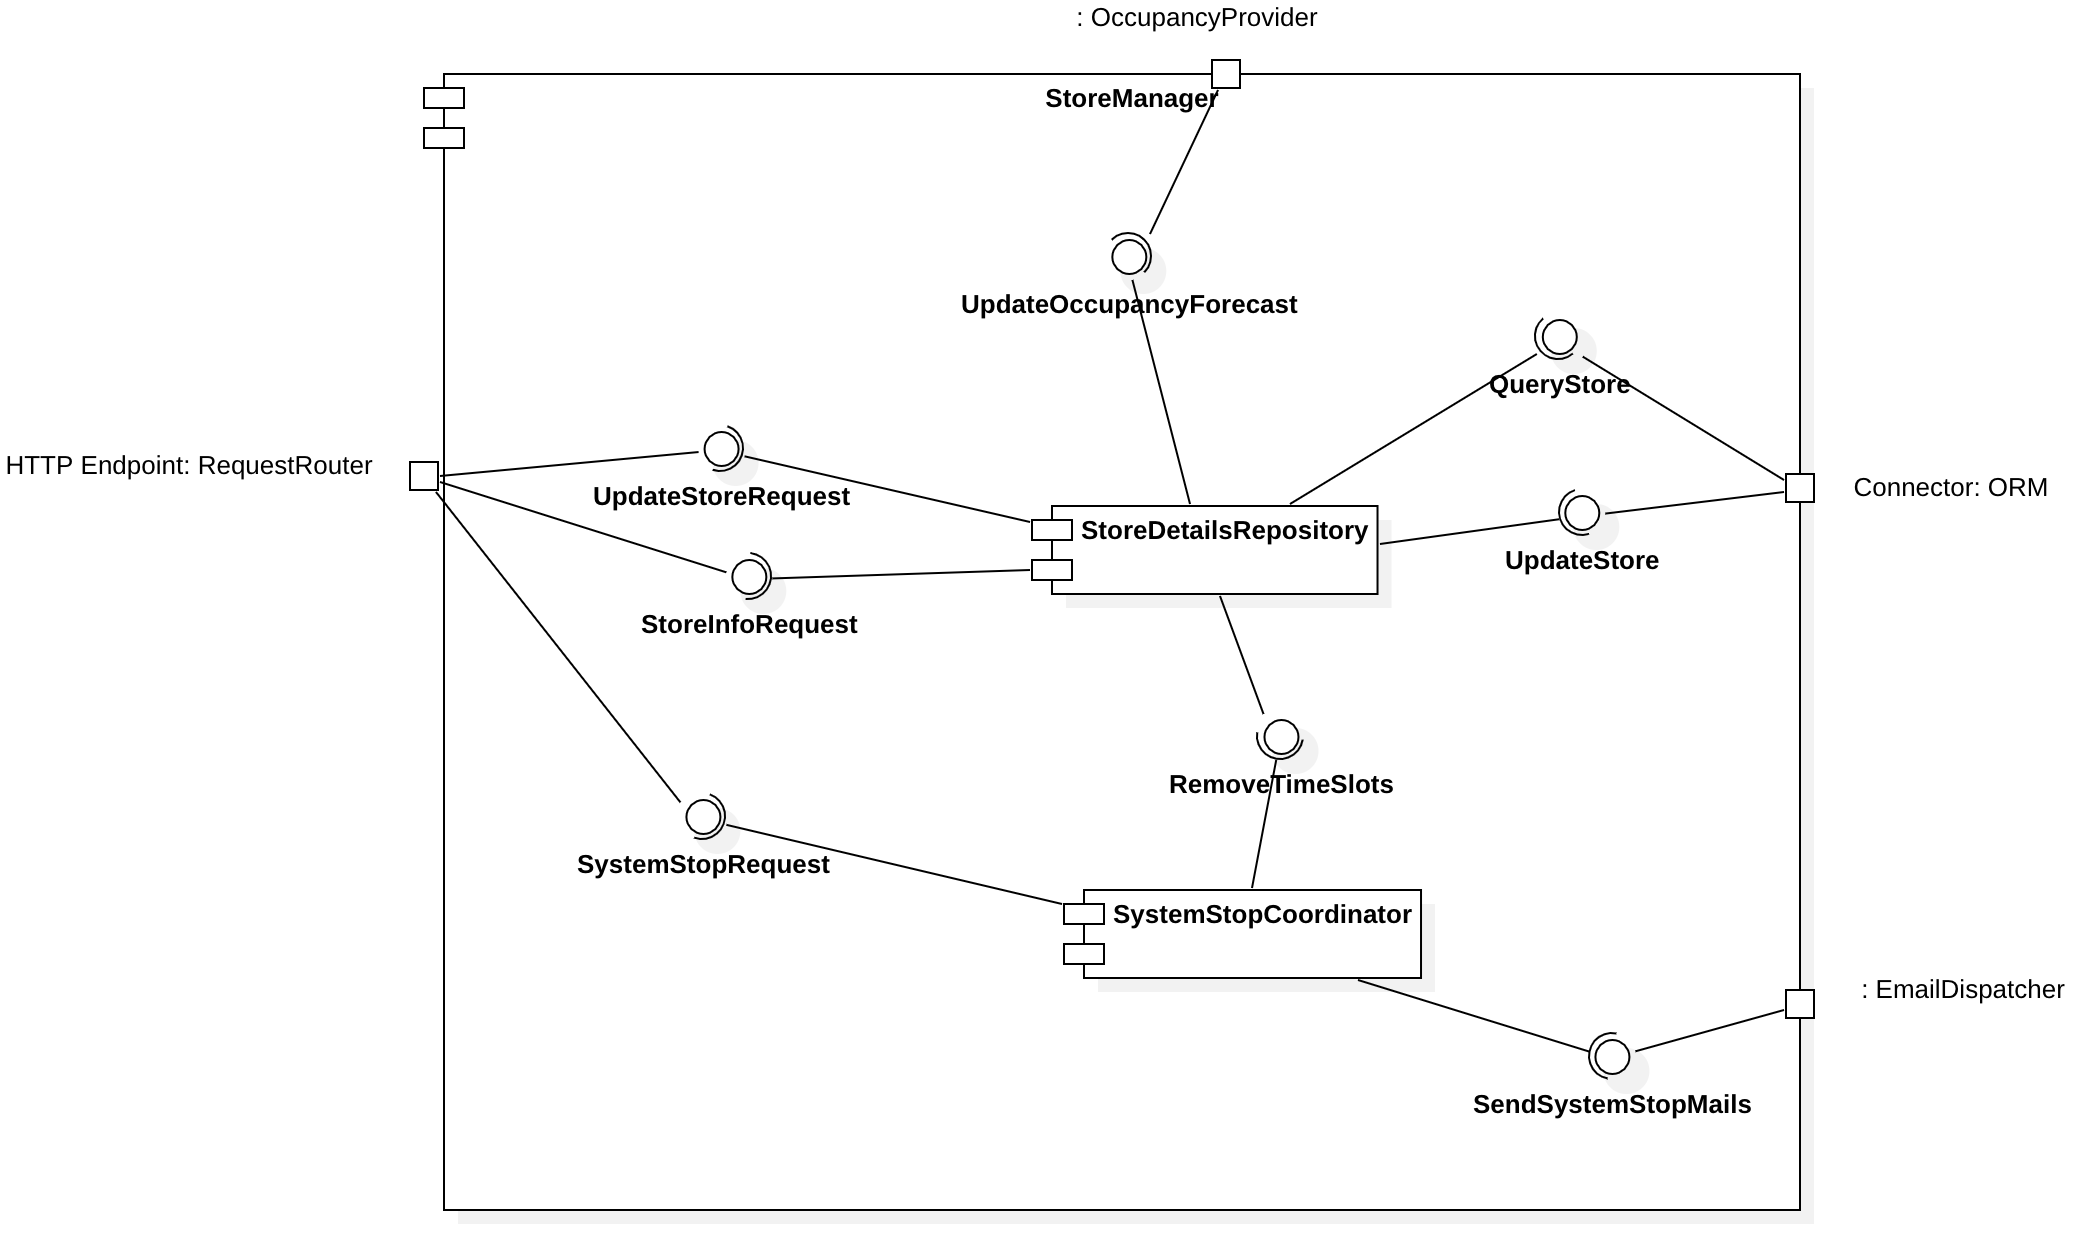
\includegraphics[height=0.4\textwidth]{Images/ComponentDiagrams/StoreManager.png}
    \caption{Component Diagram for the StoreManager}
    \label{fig:CDStoreManager}
\end{figure}
\nameref{fig:CDStoreManager} provides a detailed view over the domain component for handling requests related to the store.
The wrapping component allows querying all relevant information about the store by all, and furthermore, harbors the logic for the manager users to update different aspects related to the store, such as basic information, time slots, configuration and system stop scheduling.
This component, apart from having mailing, routing and database interfaces, exposes an interface to the OccupancyProvider to retrieve updated information about the occupancy forecast. % TODO move to subcomponent
This component is divided into following components to decrease cohesion between tasks to be performed:
\begin{itemize}
    \item \textbf{StoreDetailsRepository}: This component is responsible for carrying out any direct query to the store data and all of the included classes, which are products, categories and time slots.
    There are two exported interfaces available to be used via HTTP.
    The query interface allows all the system users to view relevant information for the store, while the manager has access to the other interface allowing them to update the information.
    The exposed interface to the OccupancyProvider allows the OccupancyForecaster to store updated information regarding the future predictions for the store.
    \item \textbf{SystemStopCoordinator}: This component is responsible for carrying out all the actions that are necessary to perform or schedule a system stop, that are removing the specific time slot and sending e-mails to customers who has already booked those time slots.
\end{itemize}

\begin{figure}[H]
\centering
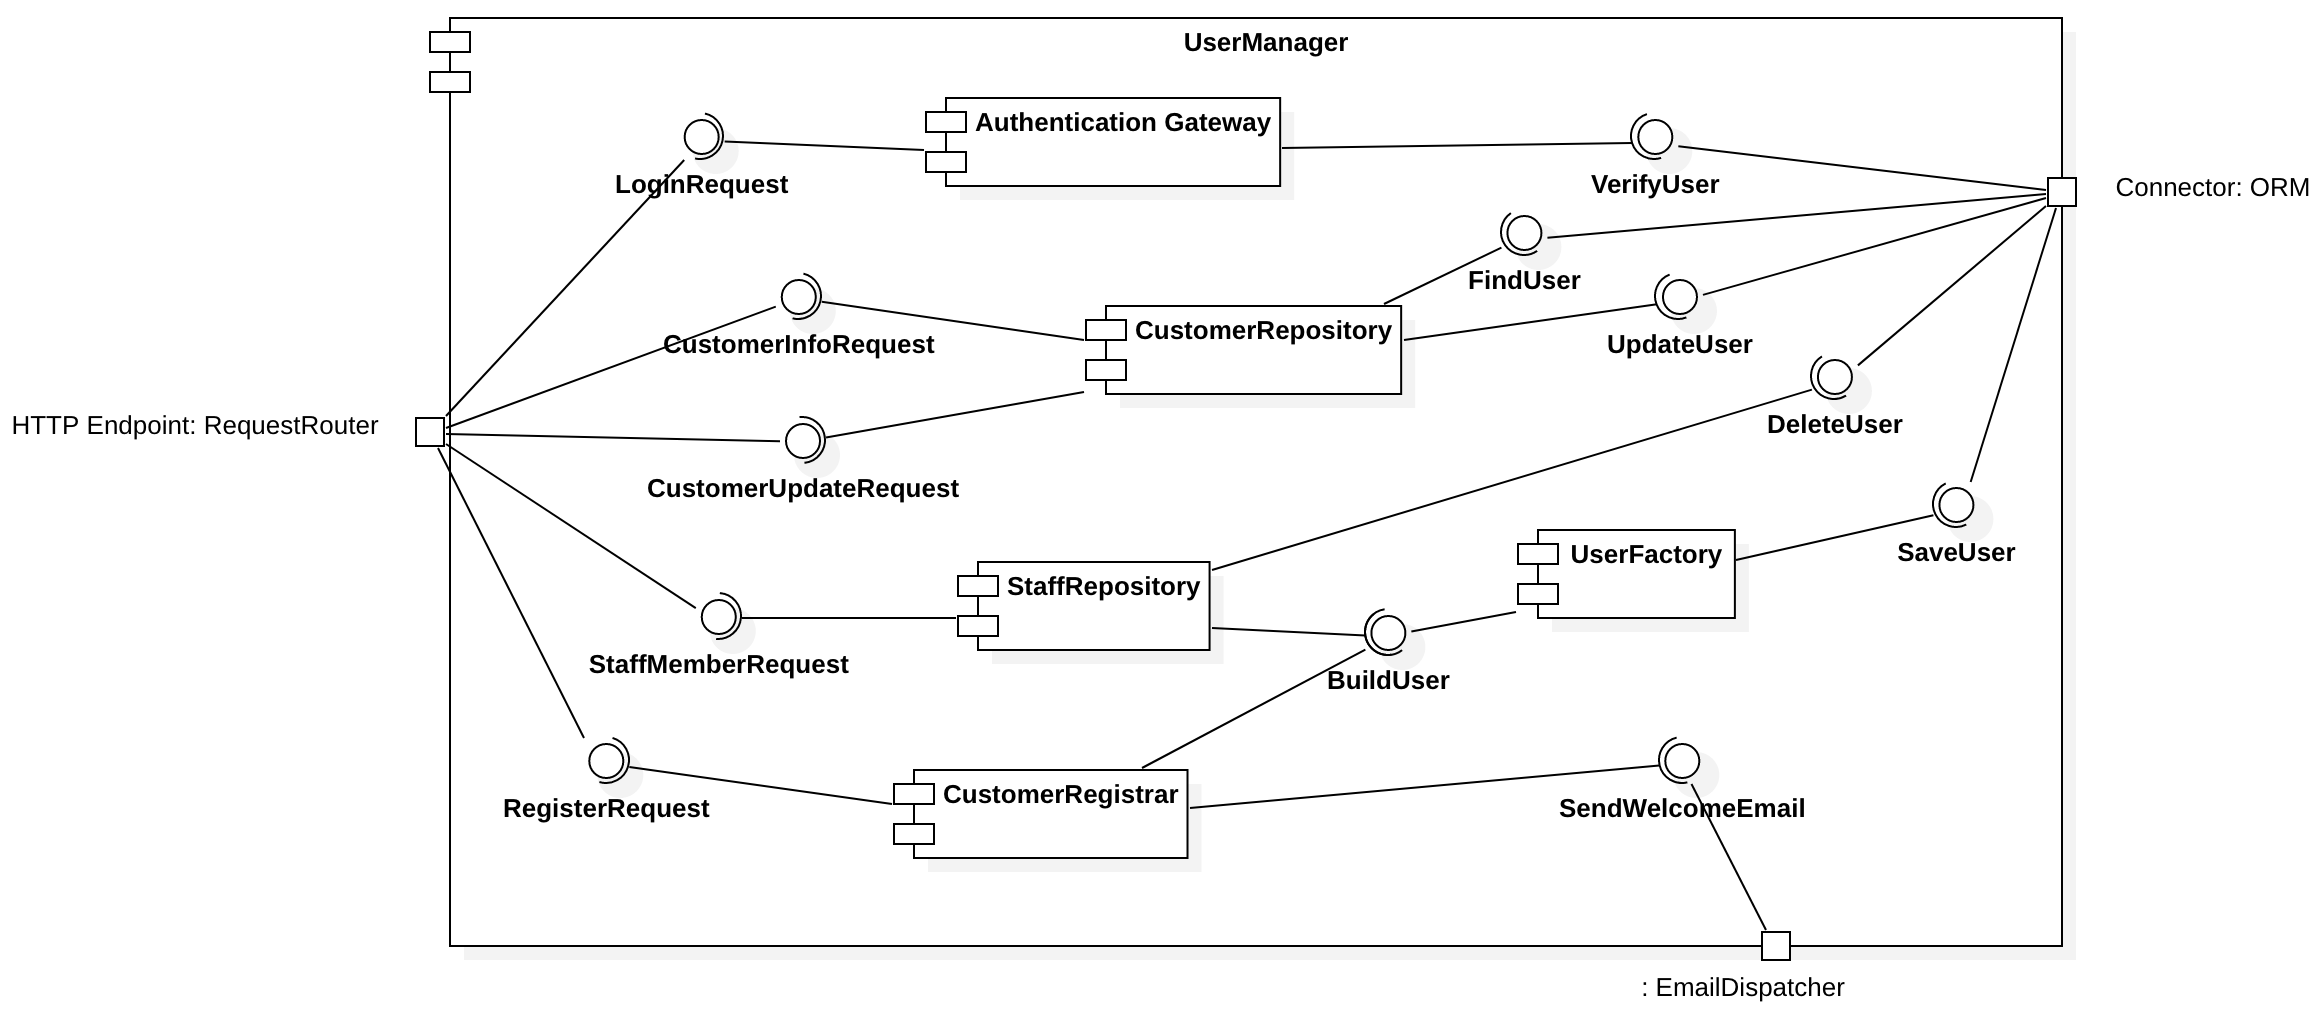
\includegraphics[height=0.4\textwidth]{Images/ComponentDiagrams/UserManager.png}
\caption{Component Diagram for the UserManager}
\label{fig:CDUserManager}
\end{figure}
\nameref{fig:CDUserManager} provides a detailed view of the sub-components related to requests that can be performed on users.
This component not only acts as a user registry, but also provides the authentication interfaces required, since its logic encompasses handling user data and authentication is done via user's email address, which relates these functions.
To seperate responsibility on different actions to be performed on the system, this component is divided into specific sub-components, that are:
\begin{itemize}
    \item \textbf{AuthenticationGateway}: This component acts as a medium to authenticate the user and generate the necessary authorization tokens for future use.
    \item \textbf{StaffRepository}: This component handles all the requests related to adding and removing staff members to stores.
    Since, in our design, different flavors of users are implemented using the same basis, the creation and removal of manager and clerks are similar from the architectural point of view.
    Furthermore, since the implementation of user creation is similar to that of the customers, a common factory component is provided to prevent duplication.
    \item \textbf{CustomerRegistrar}: This component handles the requests specific to registering new customers into the system.
    The component is responsible for calling the shared UserFactory to create a customer user and send the customer a welcome email.
    \item \textbf{UserFactory}: This component acts as a common interface and as a factory to create users.
    It is used by the components mentioned above to introduce new users to the system.
\end{itemize}
% Component diagram combining all components and each component having it's subcomponents in a different diagram with explanations
\subsection{Deployment view}
% Deployment diagram with explaining each tier
The following diagram illustrates the physical architecture and the
deployment of the system.
Each node represents a piece of hardware which harbours one or more software units.
Each piece of hardware could be replicated multiple times to improve performances as  specified in later in this document.

\begin{figure}[H]
    \centering
    \hspace*{-3.5cm}
    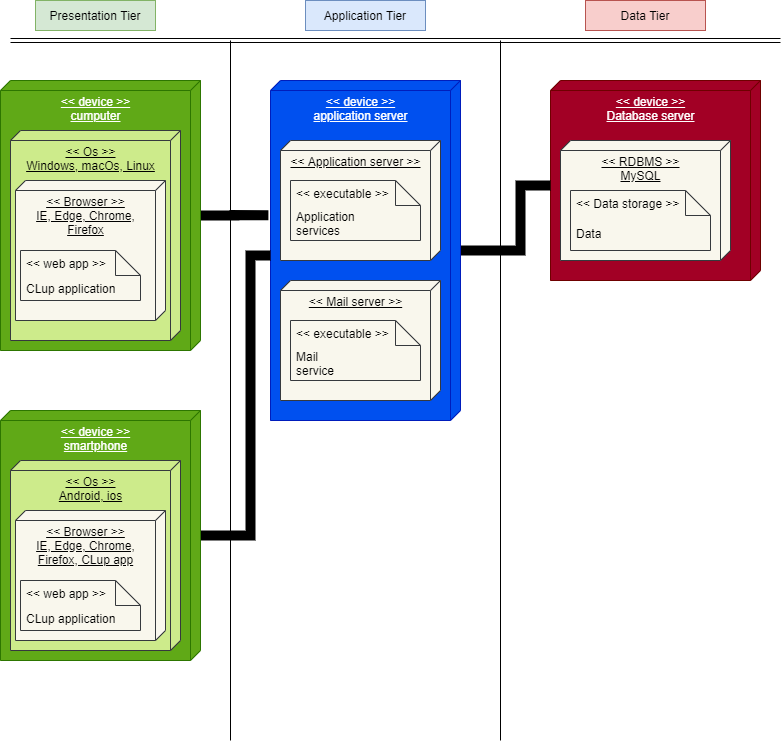
\includegraphics[height=0.7\textwidth]{Images/TierDiagram.png}
    \caption{Deployment view diagram}
\end{figure}

As shown by the diagram, this system is deployed in a three-tier
architecture, where the three tiers consist of: \\
- Presentation tier is the highest-level tier and harbours the presentation logic.
The application is thought to be a web app, so it's accessible from every device with a browser, but it's probable that
a smartphone should be the most used device to access the application so there will be android and ios applications to access
the web app.
The smartphones applications will be more similar to a browser than to a real application, therefore in the diagram is represented asa browser.
In this tier there will not be application logic, so the architecture should be thin-client.\\
- Application tier is the core level from the standpoint of logical management of the application services.
This tier contains all the application logic, from the scheduling of the line numbers to the managment of the store.
This tier is connected to the presentation tier through APIs.
An API is used for each action of the user, and the APIs are divided based on the role of the user.
Each user needs to authenticate using an API and reciving a jwt that needs to be attached to every subsequent request from the same user.
The jwt attached to the request is used to determine wich API are exposed to that user.
This tier contains also a mail Server to notify the users in case their line number is cancelled. \\

- Data tier ( tier 1 in the diagram) is the lowest-level tier as it contains all the information required to fuel the
application services, most prominently the query manager. The
databases are thought to be managed through an RDBMS
(Relational Database Management System), in particular MySQL. Relational databases
have the advantage of having near-maximum information density.
Relational constraints can improve the quality and
integrity of the content of the database.

\subsection{Runtime view}

% General TODO: Hrvoje
\subsubsection{Register}
\subsubsection{Login}
\subsubsection{Update User Information}
% Customer TODO: Roberto
\subsubsection{Book Future Line Number}
\subsubsection{Retrieve Line Number}
\subsubsection{View Store} % See location, amount of customers, if manager, more detailed monitoring
% Manager TODO: Ozan
\subsubsection{Add Staff Member}
\subsubsection{Schedule emergency Stop}
\subsubsection{Stop for Emergency}
% TODO: Ozan End
\subsubsection{Update Store Information}
% Clerk
\subsubsection{Grant Access}
\subsubsection{Generate Guest Ticket}

% You can use sequence diagrams to describe the way components interact to accomplish specific tasks typically related to your use cases

% Main use cases with sequence diagrams indicating relations of each diagram to one another.

\subsection{Component interfaces}

% Class diagram with only methods demonstrating how components interact with each other.
% Also an ER or Class diagram to indicate data.
\subsection{Selected architectural styles and patterns}
% Please explain which styles/patterns you used, why, and how
\subsection{Other design decisions}

